\documentclass{article}
\usepackage[utf8]{inputenc}
\usepackage{caption}
\usepackage[margin=1in]{geometry}
\usepackage{graphicx}
\usepackage{pdfpages}
\pdfminorversion=7

\begin{document}
\begin{titlepage}


\centering
\vspace*{2cm}
{\Huge User Interface Design Document\par}
\vspace{.25cm}
{\LARGE Course Evaluation System\par}
\vspace{1cm}
{\Large Team EVAL\par}
\vspace{.2cm}
{\Large Jovon Craig, Sam Elliott, Robert Judkins, and Stanley Small\par}
\vspace{1cm}
{\Large Client: Dr. Harlan Onsrud\par}
\vspace{1cm}
{\Large November 27, 2018\par}
\vspace{11cm}

University of Maine - Fall of 2018 - COS 397

Instructor: Professor Terry Yoo

\end{titlepage}

\newpage

\begin{center}
{
\includegraphics[scale=.2]{images/team_logo.png}} \\ 	\bigskip
{\LARGE Course Evaluation System } \\ \medskip
{\large User Interface Design Document } \\ \medskip
\end{center}

\tableofcontents

\newpage

\section{Introduction}
 

\subsection{Purpose of This Document}



\subsection{References}

Craig, J., Elliott, S., Judkins, R., \& Small, S. 29 October 2018. \textit{System Requirements Specification.}
\vspace{3mm}\newline
Craig, J., Elliott, S., Judkins, R., \& Small, S. 16 November 2018. \textit{System Design Document.}
\vspace{3mm}\newline
Fowler, M. (2004). \textit{UML Distilled: A Brief Guide to the Standard Object Modeling Language.} Boston:

Addison-Wesley.
\vspace{3mm}\newline
Onsrud, H. ``Example Question Selection Form.'' See Appendix D.

\section{User Interface Standards}


\section{User Interface Walkthrough}


\section{Data Validation}

\section{Report Formats}


\appendix

\newpage
\section{Agreement Between Customer and Contractor}
This page shows that all members of Team EVAL and the client, Harlan Onsrud, have agreed on all the information in the system design document. By signing this document, Team EVAL and Dr. Onsrud agree on the system's architecture, components, relations between the components, database schema, required files, and file descriptions.

The team will follow a process in the case that the design document is changed after we sign it. First, the team writes a rough draft of the changes to be made to the document. Second, all team members and Harlan Onsrud will sign the document agreeing to the changes. Finally, the changes are made to the final copy of the document.

\vspace{.7in}
\noindent
\begin{tabular}{ p{5cm} p{5cm} p{5cm} } 
\textbf{\textit{Name}} & \textbf{\textit{Signature}} & \textbf{\textit{Date}} \\[.5cm]
\textbf{Jovon Craig} & $\rule{5cm}{.1mm}$ & $\rule{5cm}{.1mm}$\\[.5cm]
\textbf{Sam Elliott} & $\rule{5cm}{.1mm}$ & $\rule{5cm}{.1mm}$\\[.5cm]
\textbf{Robert Judkins} & $\rule{5cm}{.1mm}$ & $\rule{5cm}{.1mm}$\\[.5cm]
\textbf{Stanley Small} & $\rule{5cm}{.1mm}$ & $\rule{5cm}{.1mm}$\\[.5cm]
\textbf{Harlan Onsrud} & $\rule{5cm}{.1mm}$ & $\rule{5cm}{.1mm}$\\[.5cm]
Customer Comments: & \multicolumn{2}{ l }{ $\rule{10.45cm}{.1mm}$ }\\[.5cm]
\multicolumn{3}{ l }{ $\rule{15.9cm}{.1mm}$ }\\[.5cm]
\end{tabular}

\newpage
\section{Team Review Sign-off}

This page shows that all members of Team EVAL have reviewed the user interface design document and agreed on its content. By signing this document, the team members agree on that all information about the system's user interface design are accurate. There is nothing in the document that is a source of contention.

\vspace{.7in}
\noindent
\begin{tabular}{ p{5cm} p{5cm} p{5cm} } 
\textbf{\textit{Name}} & \textbf{\textit{Signature}} & \textbf{\textit{Date}} \\[.5cm]
\textbf{Jovon Craig} & $\rule{5cm}{.1mm}$ & $\rule{5cm}{.1mm}$\\[.5cm]
Comments: & \multicolumn{2}{ l }{ $\rule{10.45cm}{.1mm}$ }\\[.5cm]
\multicolumn{3}{ l }{ $\rule{15.9cm}{.1mm}$ }\\[.5cm]
\textbf{Sam Elliott} & $\rule{5cm}{.1mm}$ & $\rule{5cm}{.1mm}$\\[.5cm]
Comments: & \multicolumn{2}{ l }{ $\rule{10.45cm}{.1mm}$ }\\[.5cm]
\multicolumn{3}{ l }{ $\rule{15.9cm}{.1mm}$ }\\[.5cm]
\textbf{Robert Judkins} & $\rule{5cm}{.1mm}$ & $\rule{5cm}{.1mm}$\\[.5cm]
Comments: & \multicolumn{2}{ l }{ $\rule{10.45cm}{.1mm}$ }\\[.5cm]
\multicolumn{3}{ l }{ $\rule{15.9cm}{.1mm}$ }\\[.5cm]
\textbf{Stanley Small} & $\rule{5cm}{.1mm}$ & $\rule{5cm}{.1mm}$\\[.5cm]
Comments: & \multicolumn{2}{ l }{ $\rule{10.45cm}{.1mm}$ }\\[.5cm]
\multicolumn{3}{ l }{ $\rule{15.9cm}{.1mm}$ }\\[.5cm]
\end{tabular}


\newpage
\section{Document Contributions}

Stanley Small ?? Stan contributed approximately ?? percent of the document.


Jovon Craig ??. Jovon contributed about ?? percent of the document.


Sam Elliott ??. Sam contributed about ?? percent of the document.

Robert Judkins ??. Robert contributed about ?? percent of the document.

\newpage

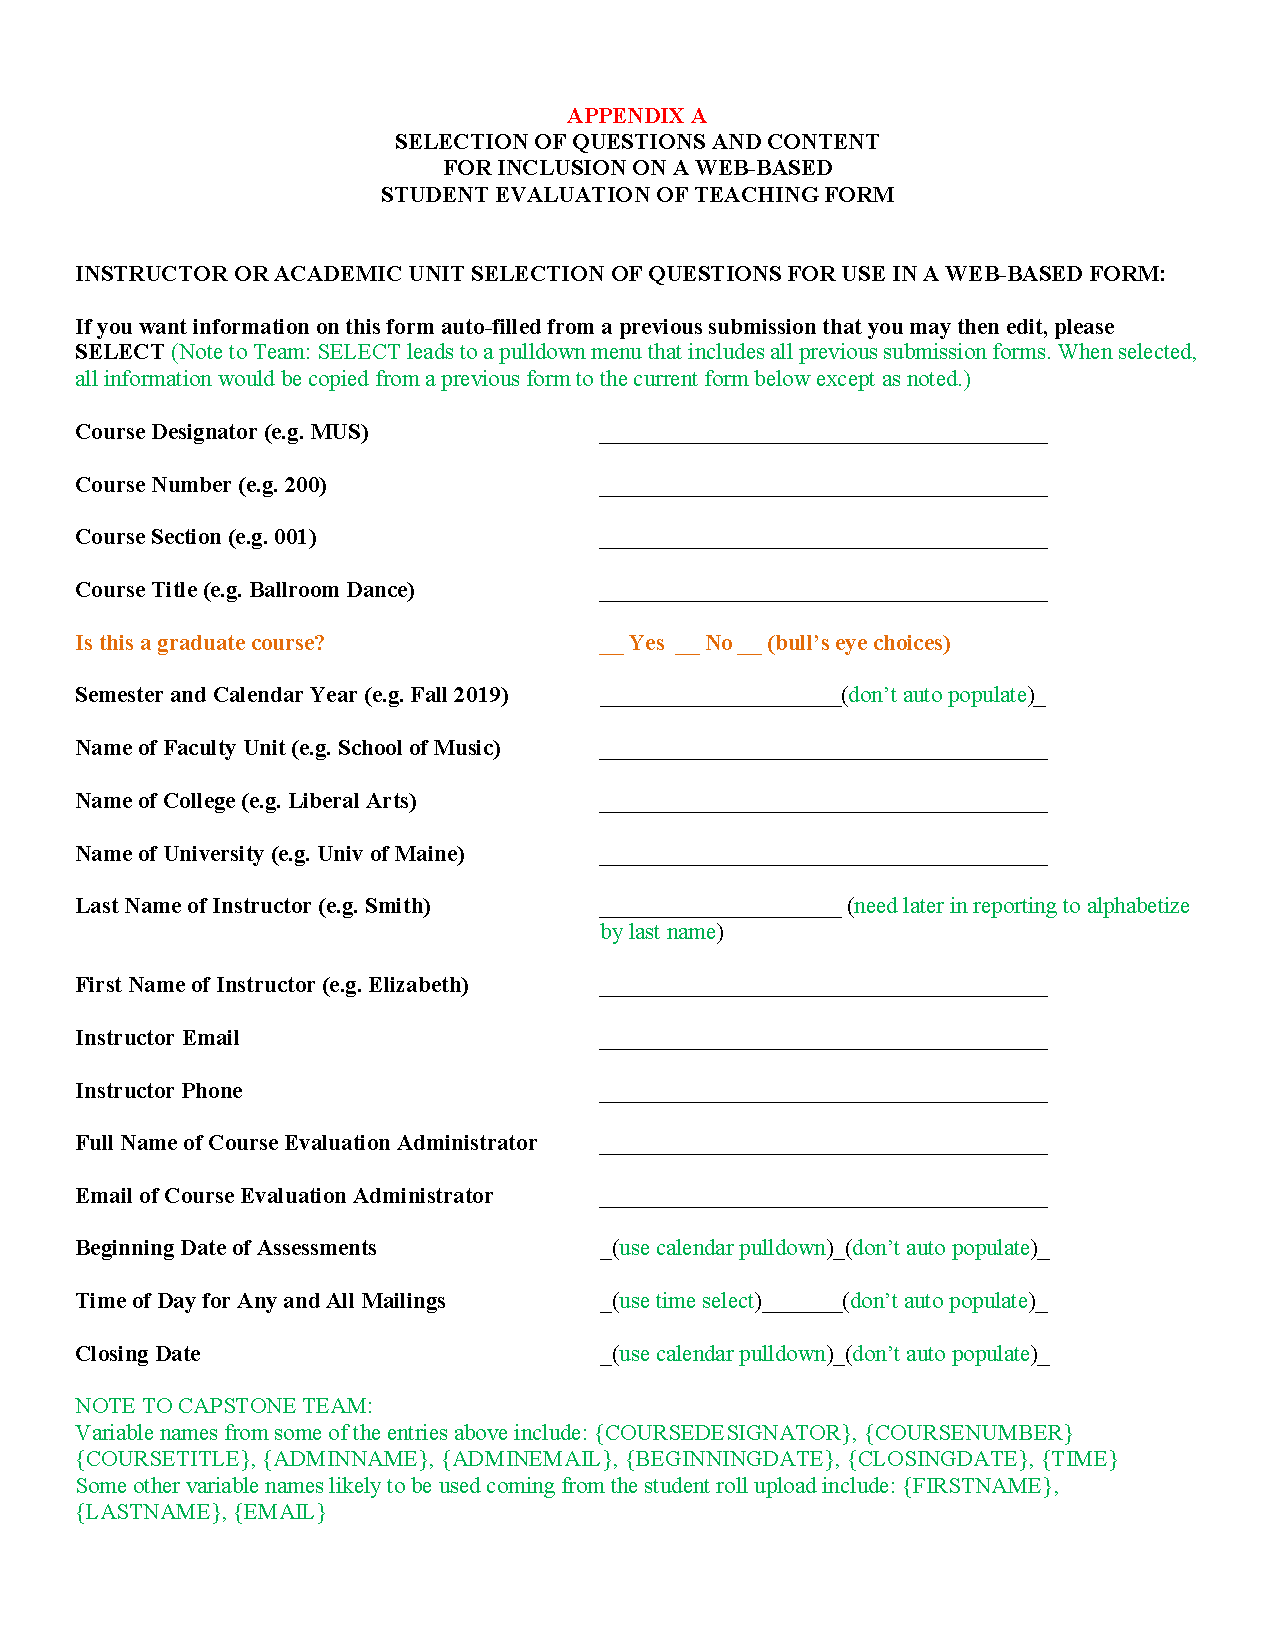
\includepdf[scale=0.85,pages=1,pagecommand=\section{Example Question Selection Form}]{images/question_appendix.pdf}
\includepdf[scale=0.85,pages=2-]{images/question_appendix.pdf}

\end{document}
